% Overall Architecture of the Proposed Method (Fig. 2)
% Compile: pdflatex framework_chart.tex -> framework_chart.pdf
\documentclass[border=4pt]{standalone}
\usepackage{tikz}
\usepackage{amsmath,amssymb}
\usetikzlibrary{shapes.geometric, arrows.meta, positioning, calc, fit, backgrounds}

\definecolor{blkblue}{HTML}{E9EEF8}
\definecolor{blkblueb}{HTML}{2B4C7E}
\definecolor{blkcream}{HTML}{FAF2E2}
\definecolor{blkcreamb}{HTML}{8C5A1E}
\definecolor{blkgreen}{HTML}{E6F5E8}
\definecolor{blkgreenb}{HTML}{2E6B35}
\definecolor{blkgray}{HTML}{F4F4F4}

\begin{document}
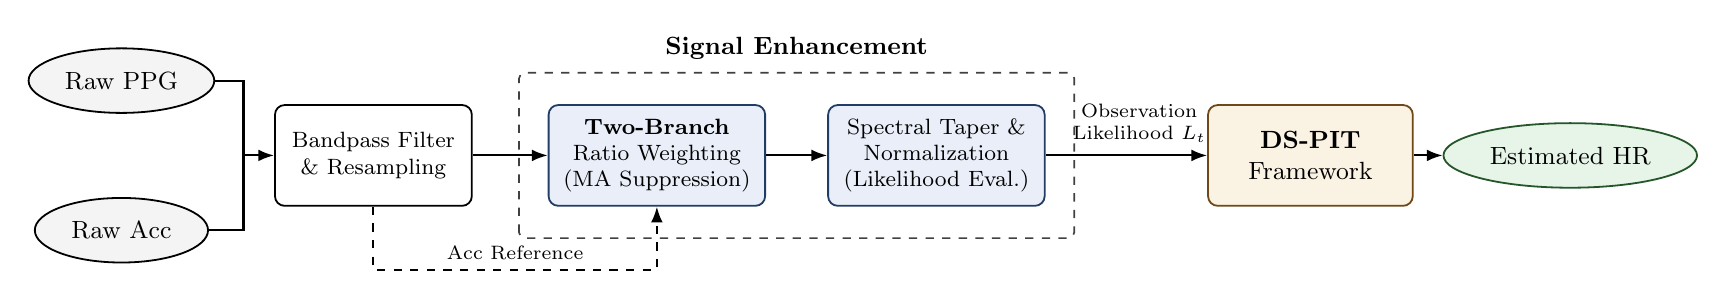
\begin{tikzpicture}[
    >={Latex[length=2.0mm,width=1.5mm]},
    arr/.style={->, draw=black, line width=0.75pt},
    darr/.style={->, draw=black, line width=0.75pt, dashed},
    io/.style={ellipse, draw=black, fill=blkgray, line width=0.65pt,
               minimum width=2.2cm, minimum height=0.82cm, align=center, font=\small},
    outnode/.style={ellipse, draw=blkgreenb!80!black, fill=blkgreen, line width=0.65pt,
                    minimum width=2.5cm, minimum height=0.82cm, align=center, font=\small},
    proc/.style={rectangle, rounded corners=3.5pt, draw=black, fill=white, line width=0.65pt,
                 minimum width=2.5cm, minimum height=1.28cm, align=center, font=\footnotesize},
    enh/.style={rectangle, rounded corners=3.5pt, draw=blkblueb!80!black, fill=blkblue, line width=0.65pt,
                minimum width=2.75cm, minimum height=1.28cm, align=center, font=\footnotesize},
    dspit/.style={rectangle, rounded corners=3.5pt, draw=blkcreamb!80!black, fill=blkcream, line width=0.65pt,
                  minimum width=2.6cm, minimum height=1.28cm, align=center, font=\small}
]

% Input nodes
\node[io] (ppg) at (0, 0.95) {Raw PPG};
\node[io] (acc) at (0, -0.95) {Raw Acc};

% Preprocessing block
\node[proc] (prep) at (3.2, 0) {Bandpass Filter\\\& Resampling};

% Signal Enhancement blocks
\node[enh] (wf) at (6.8, 0) {\textbf{Two-Branch}\\Ratio Weighting\\(MA Suppression)};
\node[enh] (norm) at (10.35, 0) {Spectral Taper \&\\Normalization\\(Likelihood Eval.)};

% DS-PIT block
\node[dspit] (dspit) at (15.1, 0) {\textbf{DS-PIT}\\Framework};

% Output node
\node[outnode] (hr) at (18.4, 0) {Estimated HR};

% Dashed container for Signal Enhancement
\draw[dashed, draw=black!75, line width=0.6pt, rounded corners=2pt]
    (5.05, -1.05) rectangle (12.1, 1.05);
\node[font=\small\bfseries, anchor=south] at (8.575, 1.10) {Signal Enhancement};

% Connections: Inputs to Preprocessing
\draw[line width=0.75pt] (ppg.east) -- (1.55, 0.95) -- (1.55, 0);
\draw[line width=0.75pt] (acc.east) -- (1.55, -0.95) -- (1.55, 0);
\draw[arr] (1.55, 0) -- (prep.west);

% Connections: Main pipeline
\draw[arr] (prep.east) -- (wf.west);
\draw[arr] (wf.east) -- (norm.west);
\draw[arr] (norm.east) -- node[above, pos=0.58, font=\scriptsize, align=center, yshift=1pt] {Observation\\Likelihood $L_t$} (dspit.west);
\draw[arr] (dspit.east) -- (hr.west);

% Reference path from Preprocessed Acc to Two-Branch Ratio Weighting
\draw[darr] (prep.south) -- (3.2, -1.45) -- node[above, font=\scriptsize] {Acc Reference} (6.8, -1.45) -- (wf.south);

\end{tikzpicture}
\end{document}
